\chapter{主序和主序后的恒星演化}\label{sec:evolution}
\section{不同质量恒星的演化}
\begin{figure}[hbt]
  \centering
  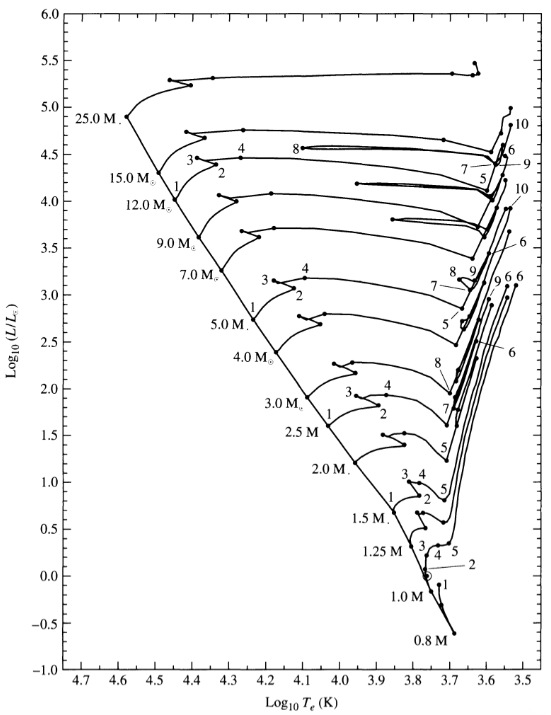
\includegraphics[width=9cm]{chapters/13/HRD}
  \caption{不同质量恒星在赫罗图上的演化}
  \label{fig:HRDM}
\end{figure}

如图\ref{fig:HRDM},不同质量的恒星在进入主序后会有不同的演化命运。可以看到,质量越大的恒星在演化过程中具有更大的温度和光度,在零龄主序处(对角斜线),光度与质量呈幂律分布(因为要满足斯特藩-玻尔兹曼定律)。

对于单个恒星的演化轨迹,一些特征区域需要注意:
\begin{itemize}
  \item 1-3,\textbf{恒星主序演化阶段},主序的定义为中心是氢燃烧阶段。显然发现恒星的主序在赫罗图上并不是简单的一条对角斜线,而是有一定的宽度。
  \item 3-5,\textbf{亚巨星支(SGB)、赫氏空隙},这是中心的氢已经全部核反应完生成了氦核,结束了主序。但是氦核周围还是充满了氢,因此这时会燃烧氦核周围的氢壳层,这会导致恒星会快速膨胀,到达最右侧的林忠四郎线轨迹。同时这里之所以称为空隙是因为恒星在这个阶段演化非常快,观测上很少能够观测到这个阶段的恒星,因此在赫罗图上形成了一段空白区域。
  \item 5-6,\textbf{红巨星支(RGB)},因为恒星膨胀到一定程度会达到平衡极限,因此之后会沿着林忠四郎线轨迹演化。这时恒星的对流区域能够达到很深的范围,会将外部物质与内部物质混合交换,被称为\textbf{第一次挖掘}。氢壳层燃烧生成氦,增加氦核的质量,并提高氦核的温度。
  \item 6-9,\textbf{氦核燃烧},通过3$\alpha$反应生成$^{12}$C。
  \item 9-10,\textbf{渐进巨星支(AGB)},氦核完全变成碳核,周围的氦壳层燃烧,恒星再次膨胀,并在此经历\textbf{第二次和第三次挖掘}。
\end{itemize}


\begin{figure}[hbt]
  \centering
  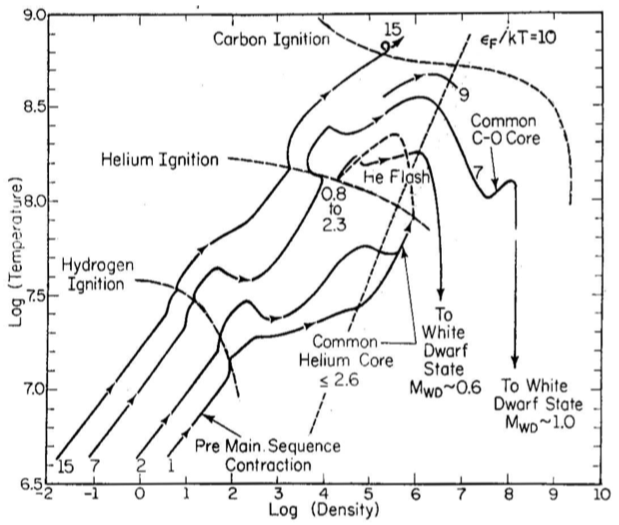
\includegraphics[width=10cm]{chapters/13/center}
  \caption{不同质量恒星中心的状态演化}
  \label{fig:center}
\end{figure}

如图\ref{fig:center},不同质量恒星在演化过程中,核心也经历了不同的命运。刚开始它们都经历了原恒星的塌缩阶段,直到中心的氢点燃,之后的演化会开始出现分歧。

$1\,M_\odot$和$2\,M_\odot$的恒星由于反应是温度和质量不够,会形成简并的氦核,然后通过氢壳层燃烧缓慢增长氦核的质量,直到氦核达到点燃温度,首先会解除氦核的简并,这一步称为\textbf{氦闪},然后稳定燃烧。

而$7\,M_\odot$和$15\,M_\odot$的恒星因为质量比较大,中心的温度会更高,在形成氦核之后温度自然达到点燃温度直接进行氦核燃烧,没有了简并的过程。这时大家都在进行氦核燃烧生成碳-氧核的过程,然后又会发生分歧。

$1\,M_\odot$、$2\,M_\odot$和$7\,M_\odot$的恒星在形成碳-氧核之后,温度不够点燃,又会发生简并,不幸的是,现在就算氦壳层的燃烧也不足以把碳-氧核的温度提高到点燃温度,它们会形成一般的\textbf{碳-氧白矮星}。

而$15\,M_\odot$的恒星能够有效的直接发生碳-氧核,甚至不发生简并阶段。

根据以上的演化过程,我们可以将恒星进行分类
\begin{itemize}
  \item 以氦核是否发生简并为界,区分小质量恒星和中等质量恒星,一般界限为$2\,M_\odot$
  \item 以碳-氧核是否发生简并为界,区分中等质量恒星和大质量恒星,一般界限为$8\,M_\odot-11\,M_\odot$
\end{itemize}

\begin{figure}[hbt]
  \centering
  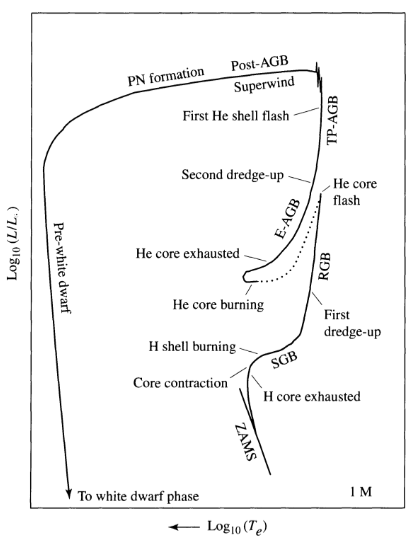
\includegraphics[width=6.4cm]{chapters/13/lowmass}
  \caption{小质量恒星的演化轨迹}
  \label{}
\end{figure}

\begin{figure}[hbt]
  \centering
  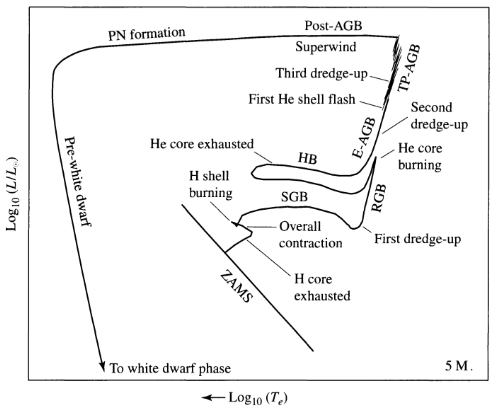
\includegraphics[width=8cm]{chapters/13/intermediate}
  \caption{中等质量恒星的演化轨迹}
  \label{}
\end{figure}

当恒星演化到渐进巨星支时,半径很大会导致表面引力束缚变弱,星风活动就会变得剧烈,引起恒星的质量损失。恒星演化到渐进巨星支后期时甚至会产生超星风,这类恒星因为在红外波段的光度最强,且能探测到羟基分子,被称为红外羟基源(OH/IR sources)。羟基分子的探测是通过羟基产生的\textbf{脉泽}实现的。脉泽即微波波段的激光,受到激发的电子从基态跃迁到第一激发态,后又退激发。但没有回到基态,而是集中在了亚稳态,当处与亚稳态的粒子集体跃迁到基态时,就产生了能量较大的微波。


\section{星团}
\subsection{星族}
恒星诞生于分子云,以星际介质为原料,而金属元素通常由恒星的核反应生成,因此恒星的分类不仅可以按照质量划分,还可以根据金属丰度来划分:
\begin{itemize}
  \item 星族III,或者第一代恒星,不含金属元素,诞生于宇宙最早期,当时的原料只有氢氦
  \item 星族II,金属丰度很低,原料基于部分第一代恒星产生的金属
  \item 星族I,金属丰度较高,最年轻的一代
\end{itemize}

\subsection{球状星团和疏散星团}
如果分子云较大,在塌缩的过程中会碎裂,分别形成恒星,这样就形成了星团。
\paragraph{球状星团}
恒星数量很多,年龄较大,分布较密集。
\paragraph{疏散星团}
恒星数量比较少,年龄较小,分布比较稀疏。

由于恒星的演化速率和质量呈正相关,质量越大,恒星的演化速度越快,因此可以通过如图\ref{fig:cluster}星团内恒星的演化来分析星团的年龄。
\begin{figure}[hbt]
  \centering
  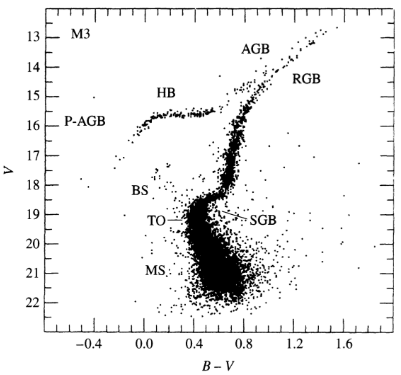
\includegraphics[width=6cm]{chapters/13/cluster}
  \caption{星团的颜色-星等图,等价于赫罗图。由于星团内恒星几乎同时诞生,质量越大,越早离开主序阶段,可以根据主序带上的拐点来确定星团的年龄。}
  \label{fig:cluster}
\end{figure}

\paragraph{赫氏空隙}
人们在一些星团的颜色-星等图中发现,主序阶段和红巨星阶段的恒星分布之间并不连续,两者之间的恒星分布很少,在图中形成了较空白的区域,这被称为赫氏空隙。赫氏空隙的产生是由于恒星在亚巨星支上的演化是热力学时标,很快就过去了,于是留下个空隙。

